% This is "sig-alternate.tex" V2.0 May 2012
% This file should be compiled with V2.5 of "sig-alternate.cls" May 2012
%
% This example file demonstrates the use of the 'sig-alternate.cls'
% V2.5 LaTeX2e document class file. It is for those submitting
% articles to ACM Conference Proceedings WHO DO NOT WISH TO
% STRICTLY ADHERE TO THE SIGS (PUBS-BOARD-ENDORSED) STYLE.
% The 'sig-alternate.cls' file will produce a similar-looking,
% albeit, 'tighter' paper resulting in, invariably, fewer pages.
%
% ----------------------------------------------------------------------------------------------------------------
% This .tex file (and associated .cls V2.5) produces:
%       1) The Permission Statement
%       2) The Conference (location) Info information
%       3) The Copyright Line with ACM data
%       4) NO page numbers
%
% as against the acm_proc_article-sp.cls file which
% DOES NOT produce 1) thru' 3) above.
%
% Using 'sig-alternate.cls' you have control, however, from within
% the source .tex file, over both the CopyrightYear
% (defaulted to 200X) and the ACM Copyright Data
% (defaulted to X-XXXXX-XX-X/XX/XX).
% e.g.
% \CopyrightYear{2007} will cause 2007 to appear in the copyright line.
% \crdata{0-12345-67-8/90/12} will cause 0-12345-67-8/90/12 to appear in the copyright line.
%
% ---------------------------------------------------------------------------------------------------------------
% This .tex source is an example which *does* use
% the .bib file (from which the .bbl file % is produced).
% REMEMBER HOWEVER: After having produced the .bbl file,
% and prior to final submission, you *NEED* to 'insert'
% your .bbl file into your source .tex file so as to provide
% ONE 'self-contained' source file.
%
% ================= IF YOU HAVE QUESTIONS =======================
% Questions regarding the SIGS styles, SIGS policies and
% procedures, Conferences etc. should be sent to
% Adrienne Griscti (griscti@acm.org)
%
% Technical questions _only_ to
% Gerald Murray (murray@hq.acm.org)
% ===============================================================
%
% For tracking purposes - this is V2.0 - May 2012

\documentclass{sig-alternate}
\usepackage{url}
\usepackage{multirow}

\begin{document}
%
% --- Author Metadata here ---
\conferenceinfo{WWW}{'15 Florence, IT}
%\CopyrightYear{2007} % Allows default copyright year (20XX) to be over-ridden - IF NEED BE.
%\crdata{0-12345-67-8/90/01}  % Allows default copyright data (0-89791-88-6/97/05) to be over-ridden - IF NEED BE.
% --- End of Author Metadata ---

\title{User sessions identification based on strong regularities in inter-activity time}
%
% You need the command \numberofauthors to handle the 'placement
% and alignment' of the authors beneath the title.
%
% For aesthetic reasons, we recommend 'three authors at a time'
% i.e. three 'name/affiliation blocks' be placed beneath the title.
%
% NOTE: You are NOT restricted in how many 'rows' of
% "name/affiliations" may appear. We just ask that you restrict
% the number of 'columns' to three.
%
% Because of the available 'opening page real-estate'
% we ask you to refrain from putting more than six authors
% (two rows with three columns) beneath the article title.
% More than six makes the first-page appear very cluttered indeed.
%
% Use the \alignauthor commands to handle the names
% and affiliations for an 'aesthetic maximum' of six authors.
% Add names, affiliations, addresses for
% the seventh etc. author(s) as the argument for the
% \additionalauthors command.
% These 'additional authors' will be output/set for you
% without further effort on your part as the last section in
% the body of your article BEFORE References or any Appendices.

\numberofauthors{7} %  in this sample file, there are a *total*
% of EIGHT authors. SIX appear on the 'first-page' (for formatting
% reasons) and the remaining two appear in the \additionalauthors section.
%
\author{
% You can go ahead and credit any number of authors here,
% e.g. one 'row of three' or two rows (consisting of one row of three
% and a second row of one, two or three).
%
% The command \alignauthor (no curly braces needed) should
% precede each author name, affiliation/snail-mail address and
% e-mail address. Additionally, tag each line of
% affiliation/address with \affaddr, and tag the
% e-mail address with \email.
%
% 1st. author
\alignauthor Aaron Halfaker\\\
       \affaddr{Wikimedia Foundation}\\
       \email{ahalfaker@wikimedia.org}
% 2nd. author
\alignauthor Oliver Keyes\\
       \affaddr{Wikimedia Foundation}\\
       \email{okeyes@wikimedia.org}
% 3rd. author
\alignauthor Daniel Kluver\\
       \affaddr{GroupLens Research}\\
       \affaddr{University of Minnesota}\\
       \email{kluver@cs.umn.edu}
\and  % use '\and' if you need 'another row' of author names
% 4th. author
\alignauthor Jacob Thebault-Spieker\\
       \affaddr{GroupLens Research}\\
       \affaddr{University of Minnesota}\\
       \email{thebault@cs.umn.edu}
% 5th. author
\alignauthor Tien Nguyen\\
       \affaddr{GroupLens Research}\\
       \affaddr{University of Minnesota}\\
       \email{nguy1749@umn.edu }
% 6th. author
\alignauthor Anuradha Uduwage\\
       \affaddr{GroupLens Research}\\
       \affaddr{University of Minnesota}\\
       \email{uduwage@cs.umn.edu}
}
% There's nothing stopping you putting the seventh, eighth, etc.
% author on the opening page (as the 'third row') but we ask,
% for aesthetic reasons that you place these 'additional authors'
% in the \additional authors block, viz.
\additionalauthors{Additional authors: Morten Warncke-Wang (GroupLens Research,
email: {\texttt{morten@cs.umn.edu}}) and Kennith Shores (GroupLens Research, email: {\texttt{shores@cs.umn.edu}}).}
\date{10 November 2014}

\newcommand{\FIXME}[1]{[\textbf{FIXME}: \textit{#1}]}

\newcommand\leadin[1]{%
	\vskip 5pt \noindent\textbf{#1.} %
}
\newcommand\leadinx[1]{%
	\vskip 5pt \noindent\textbf{#1} %
}


\maketitle
\begin{abstract}

\end{abstract}

% A category with the (minimum) three required fields
\category{H.4}{Information Systems Applications}{Miscellaneous}
%A category including the fourth, optional field follows...
\category{D.2.8}{Software Engineering}{Metrics}[complexity measures, performance measures]

\terms{Theory}

\keywords{User session}

\section{Introduction}
\label{sec:introduction}
In 2012, we had an idea for a measurement strategy that would bring insight into understand a online community.  While studying the nature of participation in Wikipedia, the open, collaborative encyclopedia, we found ourselves increasingly curious about the amount of time that volunteer contributors invested into the encyclopedia's construction.  While past work had relied on counting the number of contributions made by a user\footnote{"Wikipedian is first to hit 1 million edits" \url{http://www.dailydot.com/news/wikipedian-first-1-million-edits}} as a measure of investment, we felt that the amount of time a user invested into editing might more accurately measure investment.  This supposition was inspired by past work attempting to estimate the amount of time invested into Wikipedia as a whole\cite{clay shirky's 100 million hours}.

The measurement strategy we came up with is based on the clustering of Wikipedia editors' activities into edit sessions with the assumption that the duration of an edit session would represent a lower bound of the amount of time invested into Wikipedia contributions\cite{geiger13using}.  While we found the notion of work sessions to be intuitive from our ethnographic work in Wikipedia, we did not find a consensus in the literature for how to identify sessions from timestamped user activities.  So, we looked to the data itself for insight on what might be a reasonable approach splitting users' editing activity into sessions. The regularities we found in inter-activity time amazed us with their intuitiveness and the simplicity of session demarcation implied. It is that work that lead us to look for such regularities in other systems and to write this paper to share our results.

We are not the first to try our hands at trying to identify a reasonable way to measure user session behavior in human-computer interaction.  User sessions have been used extensively to generate metrics for understanding the performance of information resources\cite{govseva2006empirical} -- especially in the domain of search[cite cite cite] and content personalisation\cite{spiliopoulou2003framework,gomory1999analysis}. Despite this interest in understand the nature and manifestation of user sessions, no clear consensus has emerged.  In fact, some work has gone as far as arguing that sessions don't actually exist as a useful divide for user activity\cite{jones2008beyond} and that the strategy of choosing a global inactivity threshold is arbitrary\cite{montgomery2001identifying}.

In this paper, we will propose and demonstrate a strategy for identifying user sessions from log data and demonstrate that the strategy works consistently across many different types systems and user activity.  We'll start by summarizing previous work trying to make sense of user session behavior from log data.  We'll also discuss theoretical arguments about how intuitive user behavior (e.g. tasks and sessions) ought to manifest in the data. Next, we'll discuss a generalized version of the session threshold identification strategy we developed in \cite{geiger13using} and present strategies for fitting this strategy to new data.  Then, we'll introduce 6 different systems from which we have extracted 12 different logged user action types for analysis and comparison. Finally, we'll conclude with discussions of the regularities and irregularities between datasets and what that might imply for both our understanding of human behavior and the measurement of it.


\section{Related work}
\subsection{Human activity sessions}
\label{sec:human_activities}
The concept of an activity session is an intuitive one, but it's surprisingly difficult to tie down a single definition of what a session is, and how it can be demarcated.  A ``session'' may refer to ``(1) a set of queries to satisfy a single information need (2) a series of successive queries, and (3) a short period of contiguous time spent querying and examining results.''\cite{jones2008beyond}
(1) is referred to, particularly in search-related literature,\cite{jones2008beyond, eickhoff2014lessons} not as a session but as a task - a particular information need the user is trying to fulfil.  Multiple tasks may happen in a contiguous browsing period, or a single task may be spread out over multiple periods.
(2) is unclear. It may refer to a series of contiguous but unrelated queries (in which case it is identical to the third definition), or a series of contiguous queries based on the previous query in the sequence (in which case it is best understood as a sequence of tasks).
(3) is the most commonly-used definition in the literature we have reviewed\cite{spiliopoulou2003framework,white2010assessing,govseva2006empirical,nadjarbashi2004improving} This contrasts with tasks (you can have multiple tasks in a session, or multiple sessions to a single task) and is the definition of ``session'' that we have chosen for this paper. It's also the W3C definition.\cite{W3C1999}

We found inspiration in thinking about how to model user session behavior in both the empirical modeling work of cognitive science and the theoretical frameworks of human consciousness as applied to ``work activities''.
 
The lack of purely random distribution in the time between human behavior has been the topic of recent studies focusing on the cognitive capacity of humans as information processing units.  Notably, Barbasi showed that, by modeling the activities with decision-based priority queues, he could show evidence for a mechanism to explain the heavy tail in time between activities\cite{barabasi2005origin} -- a pattern he describes as bursts of rapid activity followed by long periods of inactivity.  Wu et al. built upon this work to argue that sort-message communication patterns could be better described by a ``bimodal'' distribution characterized by Poisson-based initiation of tasks and a powerlaw of time inbetween task events\cite{wu2010evidence}.

Nardi calls out the related cognitive science work for neglecting context in work patterns, motivation and community membership -- thereby inappropriately reducing a human to a processing unit in a vacuum\cite{nardi1996context}(p21).  Instead, Nardi draws from the framework of Activity Theory(AT) to advocate for an approch to understanding human-computer interaction as a conscious procession of activities.  AT describes activities as a goal-directed or purposeful interaction of a subject with an object through the use of tools. AT further formalizes an activity as a collection of actions directed towards completing the activity's goal.  Similarly, actions are composed of operations, a fundamental, indivisible, and unconscious movement that humans make in the service of performing an action.

For example application of AT, let's examine Wikipedia editing.  Our ethnographic work with Wikipedia editors suggests that it is common to set aside time on a regular basis to spend doing ``wiki-work''.  AT would conceptualize this wiki-work overall as an \emph{activity} and each unit of time spent engaging in the wiki-work as an activity phase -- though we prefer the term ``activity session''.

The \emph{actions} within an activity session would manifest as individual edits to wiki pages representing contributions to encyclopedia articles, posts in discussions and messages sent to other Wikipedia editors.  These edits involve a varied set of \emph{operations}: typing of characters, copy-pasting the details of reference materials, scrolling through a document, reading an argument and eventually, clicking the ``Save'' button.

In this work we draw from both the concepts of the operation-action-activity heirarchy of Activity Theory and the empirical modeling strategies of cognitive science as applied to time between events.


\subsection{Session identification}
\label{sec:session_identification}
User sessions have been used as behavioral measures of human-computer interaction for almost two decades, and for this reason, strategies for session identification of log data has been the extensively studied\cite{eickhoff2014lessons}.

Cooley et al.\cite{cooley1999data} and Spiliopoulou et al.\cite{spiliopoulou2003framework} contast two primary strategies for identifying sessions from activity logs: ``navigation-oriented heuristics'' and ``time-oriented Heuristics''.  Time-oriented heuristics refers to the assignment of a inactivity threshold between logged activites to serve as a session delimiter.  The assumption here is that if there is a break between a user's actions that is sufficiently long, it's likely that the user is no longer \emph{active}, the session is assumed to have ended, and a new session is created when the next action is performed. This is the most commonly used approach to identify sessions, with 30 minutes as the most commonly used threshold\cite{spiliopoulou2003framework,eickhoff2014lessons,ortega2010differences}.  Both threshold and approach appear to originate in a 1995 paper by Catledge \& Pitkow\cite{catledge1995characterizing} that used client-side tracking to identify browsing behaviour. In their work, they reported that the mean time between user observed user events in their data was 9.3 minutes.  They choose to add 1.5 standard deviations to that mean to achieve a 25.5 minutes inactivity threshold.  Over time this proposed inactivity threshold has gradually been smoothed out to 30 minutes.  The utility of the 30-minute threshold is widely debated; Mehrzadi \& Feitelson (2012) \cite{mehrzadi2012onextracting} found that 30 minutes produced artefacts around long sessions, and could find no clear evidence of a natural session inactivity threshold\footnote{Note that this conclusion was reached using the same AOL search dataset that we analyze in this paper.}, while Jones \& Klinkner\cite{jones2008beyond} found the 25.5 minute threshold ``no better than random'' in the context of search tasks. Other thresholds have been proposed, but Montgomery and Faloutsos\cite{montgomery2001identifying} concluded that the actual threshold chosen made little difference to its accuracy.

Referer-based reconstruction involves taking the referers and URLs associated with each request by a user, and chaining them together. When a user begins navigating without a referer, they have started a session; when a trail can no longer be traced to that request based on the referers and URLs of subsequent requests, the session has ended.  This approach was pioneered by Cooley et al in 2002\cite{cooley1999data}.  While it demonstrated utility in identifying ``tasks'', and has been extended by Nadjarbashi-Noghani et al.\cite{nadjarbashi2004improving} it shows poor performance on sites with framesets due to implicit assumptions about web architecture\cite{berendt2003impact}. The sheer complexity of this strategy and it's developmental focus on \emph{task} over \emph{session} make it unsuitable as a replacement for time-oriented heuristics in practical web analytics.

In our this work, we'll challenge the conclusions of prior works' assertions (1) that no reasonable cutoff is from the empirical data and (2) that a global inactivity threshold is inappropriate as a session identification strategy.  To our knowledge, we are the first to apply a general session identification methodology to a large collection of datasets and conclude that not only are global inactivity thresholds an appropriate strategy for session identification, but also that, for most user-initiated actions, an inactivity threshold of 1 hour is appropriate.


\section{Methods}
\label{sec:methods}
This section is intended to both serve as a description of our methodology as well as to instruct readers on how to apply the same methods to their own dataset.  First, we'll discuss how we recommend applying our methodology for identifying inter-activity type component clusters to a dataset.  Next, we'll describe the origin of our datasets and the cleanup we performed in order to generate inter-activity times to fit.

\subsection{Fitting inter-activity times}
First, we must gather a dataset of user-initiated actions with timestamps of at least seconds resolution.  We generate inter-activity times on a per-user basis, so a relatively robust user identifier is necessary.  While a persistent user identifier such as one associated with a user account is preferable, we've found that, in the case of request logs, a fingerprint based on the request's IP and User-agent seems to be sufficient.

Once we have per-user inter-activity times, we plot a histogram based on the logarthmically scalled iter-activity time and look for evidence of a valley.  Given the observations we have seen (and report in section \ref{sec:results}), we expect to see a valley around about 1 hour with peaks around 1 minute and 1 day.  It's at this time that anomalies in the data should be detected and removed.  For example, we found that the time between Wikimedia Mobile Views (described in the next section) had an absurd spike at exactly 18 minutes of inter-activity time caused by a few (likely automated) users and removed their activities from the dataset.

Next, we try to fit a two component gaussian mixture model using expectation maximization\cite{benaglia2009mixtools} and visually inspect the results\footnote{Note that we tried several strategies for statistically confirming the most appropriate fit -- of which we found Davies--Bouldin index (DBI)\cite{davies1979cluster} to be most reasonable -- but none were as good as a simple visual inspection, so we employ and recommend the same.}  When the simple bimodal components did not appear to fit the data appropriately, we explored the addition of components to the mixture model with careful skepticism and repeated visual inspection.

Finally, if we have found what appears to be an appropriate fit, we identify a theoretically optimal inter-activity threshold for identifying sessions by finding the point where inter-activity time is equally likely to be within the gaussians fit with sub-hour means (within-session) and gaussians fit with means beyond an hour (between-session).

\subsection{Datasets}
\FIXME{Oliver writes up dataset descriptions}


\section{Results \& discussion}
\label{sec:results_and_discussion}
\begin{figure}
\centering
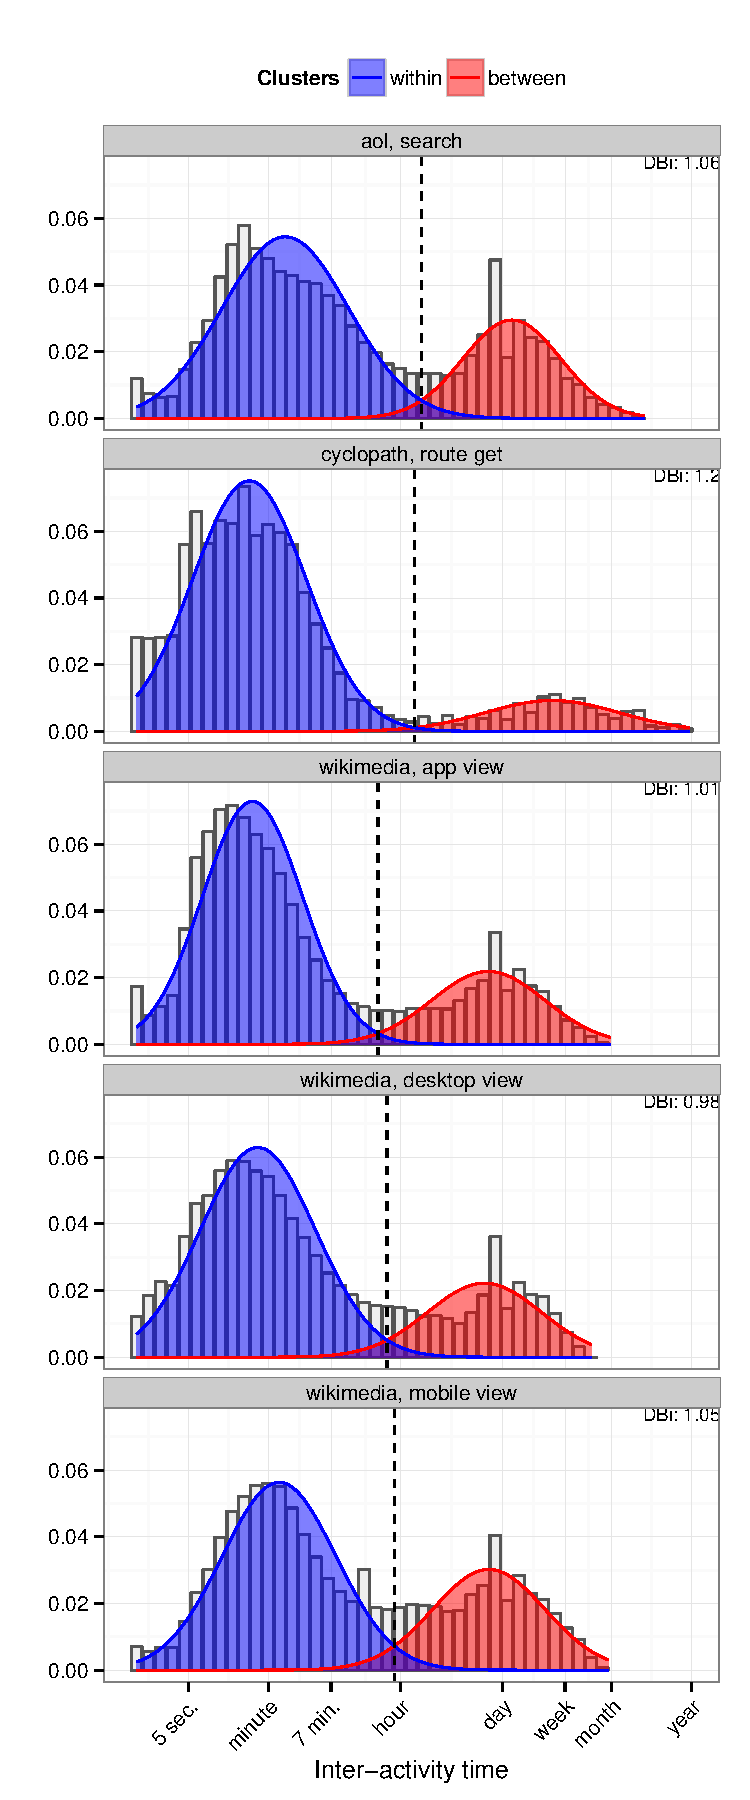
\includegraphics[width=.45\textwidth]{figures/bimodal_clusters.pdf}
\caption{
    \textbf{Bimodal clusters.} Empirical inter-activity density (bars) and fitted mixture models of gaussians are plotted for datasets where two clusters appeared to sufficiently explain the observed data.
}
\end{figure}
\input{tables/bimodal_fits}
In this section, we present and discuss the result of the application of our proposed inactivity threshold identification analysis on the datsets.  First we start off with the common, simple cluster fits.  Then we move to more complicated fits and discuss the implications of additional clusters,  Finally, we demonstrate datasets with less suitable fits and discuss what this implies about the nature of participation in these systems.

\subsection{Simple bimodal fits}
Most of the datasets of user-initiated inter-activity times that we observed display a simple bimodal distribution when their histograms are plotted on a logarithmically scaled X axis.  Figure \ref{fig:bimodal_clusters} plots a log inter-activity time histogram overlaid with expectation maximization fits of a mixture of two log-normal cluster components.  Notably, the AOL search logs represent one of the most clear fits to this bimodal distribution.  This suggests that, counter to Mehrzadi
\& Feitelson's conclusions\cite{mehrzadi2012onextracting}, there does seem to to be a clear location for an inactivity cutoff in this dataset -- at approximately one hour.

Figure \ref{fig:bimodal_clusters} demonstrates the striking regularity of inter-activity time between systems.  All of the systems presented show a clear fit for a theoretical \emph{within-session} cluster with a mode around 1 minute and a theoretical \emph{between-session} cluster with a mode at 1 day.  Each fit intersects at approximately one hour -- with Wikimedia app views display the lowest intersection at 29 minutes while AOL searches display the highest intersect at 115 minutes -- nearly two hours.   Despite this variance in the intersection points, a visual inspection of the empirical distribution does not suggest that the choice of a 1 hour cutoff for either of these datasets would be inappropriate.  Indeed, many of the \emph{between-session} clusters appear to be left shifted due to a lack of longitudinal data and it is only in these cases that the intersection falls below the one hour mark.

Also of note in these results is the spike of probability of a 24 hour inter-activity time for all but the cyclopath datasets.  This suggests that, for reading Wikimedia sites and searching in AOL, there is a strong tendency to return on a daily basis.  The curious lack of such a day-spike for cyclopath route searches could be explained by the type of usage the site sees. Bicycle route searching may be less of a daily information need than web search and Wikimedia's encyclopedia content.

\subsection{Fits with extended breaks}
\begin{figure}
\centering
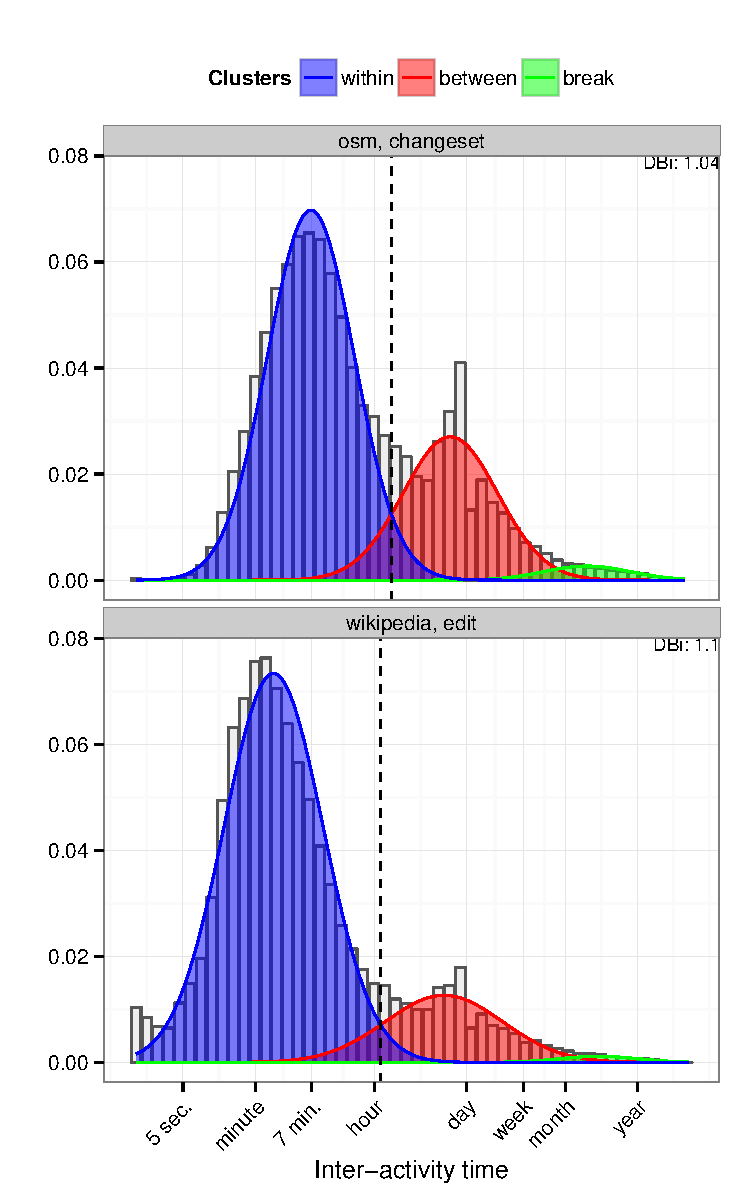
\includegraphics[width=.45\textwidth]{figures/trimodal_clusters.pdf}
\caption{
    \textbf{Trimodal clusters.} Empirical inter-activity density (bars) and fitted mixture models of gaussians are plotted for datasets where an additional, ``break'' cluster was needed to fit the data.
}
\end{figure}
In some cases, we found that the data were fit better by adding a third component to the mixture model that represents very low frequency events.  Figure \ref{fig:trimodal_clusters} shows the fits for the inter-activity time between Open Street Map's changesets and English Wikipedia edits.  Note that, like the bimodal fits above, we again see modes for the \emph{within-session} cluster around 1 minute and modes for the \emph{between-session} cluster around 1 day.  However, we found that we could more cleanly fit these datasets with an additional cluster with a mode of around 2.5 months.

As we noted in \cite{geiger13using}, we believe that this low frequency cluster represents an extended break from contributing that corresponds to a life event -- like getting married, buying a house, going to school or getting a job.  Wikipedia editors refer to this phenomena in volunteer participation as a ``wikibreak''\footnote{\url{https://en.wikipedia.org/wiki/Wikipedia:Wikibreak}}.  We suspect that the reason for the tiny scale of this cluster is two-fold: (1) contributors who work on Wikipedia or Open Street Map for long enough to to take an extended break are rare compared to other, higher frequency activity and (2) breaks often result in total abandonment of participation in the project.

\subsection{Fits with a high frequency component}
\begin{figure}
\centering
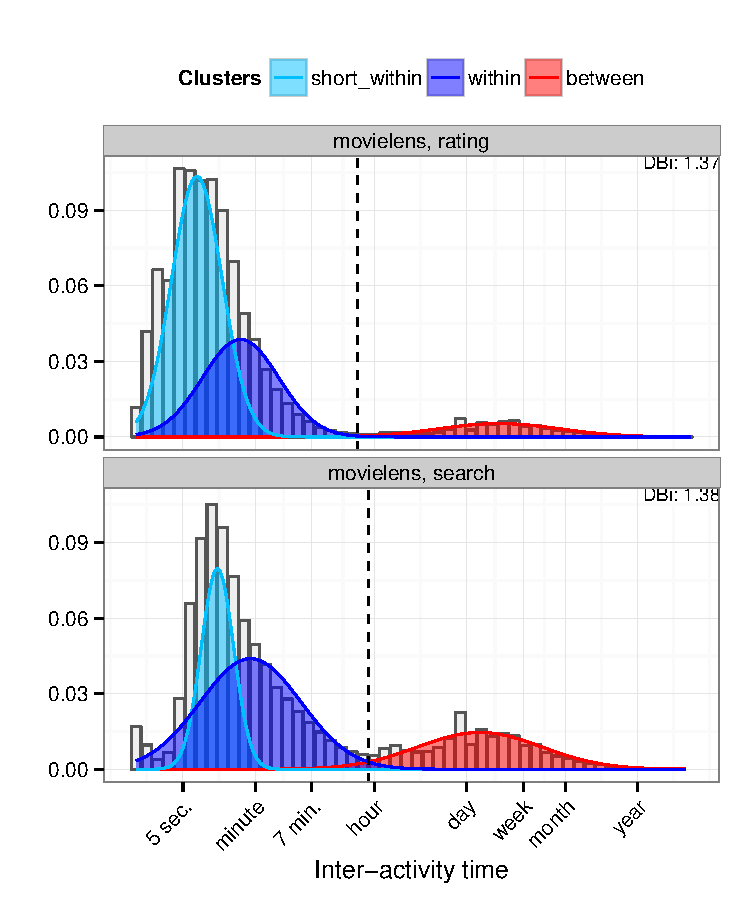
\includegraphics[width=.45\textwidth]{figures/operation_mixed_clusters.pdf}
\caption{
    \textbf{High frequency activity clusters.} Empirical inter-activity density (bars) and fitted mixture models of gaussians are plotted for datasets where an additional, high-frequency inter-activity cluster was needed to fit the data.
}
\end{figure}
When observing the distribution of inter-activity times for ratings and searches in Movielens, we found that both these events occurred with higher frequency than the other datasets.  This made us suspect that there could be an additional cluster component at a high frequency time interval.  Figure \ref{fig:mixed_operational_clusters} shows how the two datasets lent themselves to this additional ``short within'' component.  Like in previous mixture models, we see a within-session cluster with a mode around one minute and a between-session cluster with a mode around 1 day.  However, in these datasets we also observed a pattern in inter-activity times that suggested a faster component with a mode around 30 seconds.

Given that this component occurs at shorter intervals than the within-session component, we assume that it also represents within-session activity.  In the case of rating, this high frequency component could represent the rapid rating behavior that the Movielens interface affords -- a user can rate several movies from a list without leaving a page.  However, we're less sure of on how to explain the high frequency component of Movielens searches.  It could be that, unlike when performing a web search (AOL) or reading encyclopic content (Wikimedia), users' movie searches are more likely to benefit from more rapid iteration.


\subsection{Unusual fits}
\begin{figure}
\centering
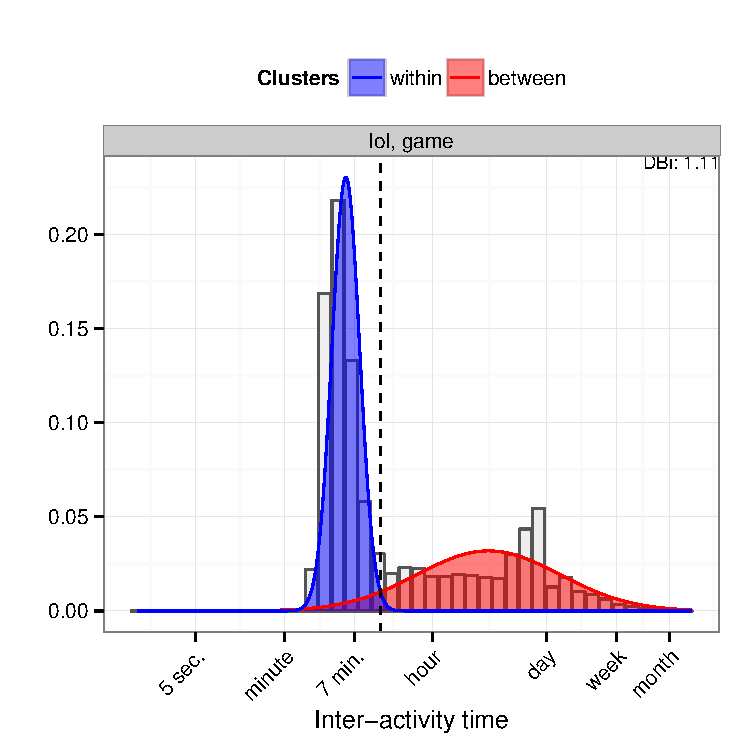
\includegraphics[width=.45\textwidth]{figures/weird_lol_clusters.pdf}
\caption{
    \textbf{Inter-game clusters.} Empirical inter-activity density (bars) and fitted mixture models of gaussians are plotted for time between League of Legends games.
}
\end{figure}
While the fits described so far follow a clear pattern with somewhat minor nuance as to the nature of the gaussian fitting strategy, the other datasets we observed suggest that the this strategy for identifying session thresholds is not universally suitable for all user-intiated events.

\leadin{League of Legends}
Figure \ref{fig:lol_game_clusters} shows the two cluster fit for League of Legends game playing.  Here, we see a very high density component with a mode around 5 minutes and a very wide component with a mode around 5 hours.  The intersection of these components place the threshold at approximately 14 minutes.  It is important to note that the tightness of the dense component may be an artifact of the way that inter-game times differ from the inter-activity times observed in the other datasets.  In the case of this dataset, only the time between games is accounted for -- not the time between game-start or game end.

There also may be constraints inherent to the system which limit the potential time spans in which a user could possibly act.  For example, League of Legends employs a queuing mechanism for matching teammates which takes approximately 5 minutes to complete at most times.  Our own experience with the game suggests that many users will finish one game and immediately get into the queue for another.  It is likely that these system limitations are the reason for infrequent between-game times under 1 minute, and understanding how systems limit user behavior is often helpful when interpreting cluster fit.

\leadin{Stack overflow}
\begin{figure}
\centering
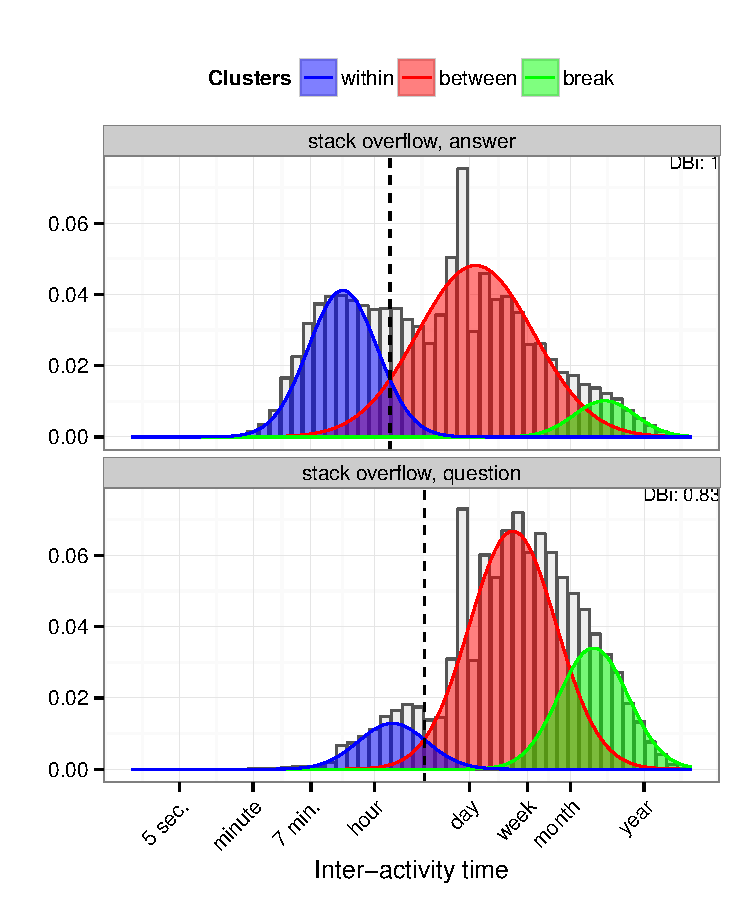
\includegraphics[width=.45\textwidth]{figures/weird_so_clusters.pdf}
\caption{
    \textbf{Low frequency clusters.} Empirical inter-activity density (bars) and (non-convergent) fitted mixture models of gaussians are plotted for time between posts on Stack Overflow.
}
\end{figure}
Unlike the other datasets observed, the time between Stack Overflow posts does not suggest a clear valley from which to draw intuition about where to draw a session cutoff.  Figure \ref{fig:stack_overflow_clusters} shows the (non-convergent) fits of question asking and answering activities.  In this case, there is a dramatic reduction in the scale of the higher frequency time components and what appears to be a shift of the within-session component to the right.

If we are to interpret the fit of these clusters as meaningful, the right shift of the within-session component could be due to the time needed to produce a high quality question or answer.  Stack Overflow's incentive structure is designed to encourage high quality posts.  High quality posts are more likely to be reviewed positively by other users, and a user's score within StackOverflow is largely dependent on how other users rate the quality of their posts\footnote{\url{http://meta.stackexchange.com/help/whats-reputation}}.  It's seems likely that producing a high quality post would take a substantial amount of time and that this time investment would make posting with a high enough frequency to produce a short inter-activity time component like we saw in other systems difficult.  In this case, it seems that either our strategy for identifying a suitable inactivity threshold is insufficient or that Stack Overflow users rarely post more than one question or answer within an activity session.


\section{Implications \& future work}
\label{sec:implications_and_future_work}
In this paper, we have challenged previous literature that suggest no apparent inactivity threshold exists for identifying user session behavior.  From this, we propose a rule of thumb and a simple methodology for checking this rule in other datasets.  The rule of thumb is simple; our analysis suggests that setting an inactivity threshold at \emph{one hour} should robust to new datasets since it is (1) grounded in empirical observations of a natural valley in activity times that corresponds to intuition and (2) holds constant across a wide range of systems and activities. Even when our threshold detection strategy deviated from one hour, the devations were relatively small given the scale of activities, and in some cases, this deviation could be explained by limitations in the data.  However, we still advise that any new application of session identification using an hour as an inactivity threshold is preceeded by a plot of a histograph of log-scaled inter-activity times and visual inspection for a natural valley between 1 minute and 1 day to confirm its suitability.

These results and our recommendations stand in the face of a long and nuanced discussion of the nature of user sessions as can be extracted from logged interactions with a computer system.  We place out criticisms of previous work into two categories: (1) empirical work that did not attempt to look for log-normally distributed patterns and therefore concluded that no obvious separation between within- and between session inter-activity times exist\cite{something}\FIXME{Oliver, can you list relevant cites here?} and (2) work exploring \emph{task driven} behavior that suggests that tasks are not well contained within a session.  We challenge (1) on the basis of the clear trends represented in the results of this work and (2) by drawing a distinction between goal-directed tasks (\emph{action} in Activity Theory) and activity sessions which often represent a collection of tasks.

Further, given the strong regularities we see between between different types of human-computer interactions, our results suggest something more fundimental about human activity itself.  As discussed in section \ref{sec:human_activity}, Activity Theory(AT) conceptualizes human consciousness as a sequence of \emph{activities} which represent a heirarchical relationship with \emph{actions} and \emph{operations}.  We suspect that the fact that \emph{operations} and \emph{actions} must be performed in a sequence may suggest a natural temporal rhythm.  While it's hard to say conclusively, we suspect that the ``short\_within'' clusters we observe represent \emph{operation}-level events, the ``within'' clusters represent \emph{action}-level events, and the ``between'' clusters represent \emph{activity}-level events.

If this application of AT to the observed patterns is accurate, that could have substantial implications for the design of design of systems.  System designers may be able to take advantage of the regularities observed by constructing systems that afford operations, actions and activity at timescales that humans will feel to be natural.  Our analysis suggests that operations should exist at the timescale of about 5-20 seconds, actions should be completable at a timescale of 1-7 minutes and activities should be supported at daily to weekly time intervals.  We suspect that systems that do not allow users to work at these time scale may be frustrating or may otherwise limit their ability of their users to function at full capacity.

These ruminations about human behavior and its manifestation in well designed systems are only speculation at this point.  New work will need to be done to explore whether our predictions hold and whether any effect is truely of substantial effect.  


\section{Acknowledgments}
\label{sec:acknowledgements}
We are tremendously grateful to Dror Feitelson for agreeing to share the AOL search dataset.


\bibliographystyle{abbrv}
\bibliography{refs}

%\balancecolumns
\end{document}
